\documentclass[11pt,letterpaper]{article}
\usepackage[margin=0.9in]{geometry}
\usepackage[T1]{fontenc}
\usepackage[utf8]{inputenc}
\usepackage{lmodern,microtype}
\usepackage{amsmath,amssymb}
\usepackage{titlesec}
\titlelabel{\thetitle:\quad}
\usepackage{booktabs,tabularx,longtable,array,float}
\usepackage[justification=centering]{caption}
\usepackage{tikz,pgfplots}
\usepgfplotslibrary{groupplots}
\pgfplotsset{compat=1.18}
\usepackage{xcolor,hyperref,listings}
\hypersetup{colorlinks=true,linkcolor=blue!55!black,urlcolor=blue!55!black}
\definecolor{utblue}{RGB}{22,67,117}
\definecolor{mutedblue}{RGB}{98,147,186}
\definecolor{warmorange}{RGB}{194,99,46}
\setlength{\parskip}{5pt}
\setlength{\parindent}{0pt}
\renewcommand{\arraystretch}{1.15}
\captionsetup{font=small,labelfont=bf}
\lstdefinestyle{rsource}{language=R,basicstyle=\ttfamily\scriptsize,breaklines=true,columns=fullflexible,commentstyle=\color{teal!65!black},keywordstyle=\color{utblue},showstringspaces=false,frame=single,rulecolor=\color{black!20},xleftmargin=0.15in,xrightmargin=0.15in}

\title{\vspace{-2cm}\bfseries Exploratory Data Analysis\\\large Factors Influencing Students' Choice of Study Location\\\normalsize STA304H5F}
\author{Luai's Fan Club \quad | \quad University of Toronto Mississauga}
\date{October 25, 2026}

\setcounter{tocdepth}{2}
\begin{document}
\maketitle
\vspace{-1cm}

\section{Data and preliminary checks}
Our target population consists of students enrolled in STA304H5F at the University of Toronto Mississauga during Fall 2026. We collected 55 survey responses, with 26 variables covering students' study locations, the factors they consider important, their academic tasks, and barriers to using their preferred study spaces.

Before starting the analysis, we checked the dataset for missing values, duplicate responses, and invalid entries. All 55 respondents provided a course-specific ID, and no duplicate IDs were found. All numerical responses were within the expected 1–7 scale, so no responses were removed. There were also two written responses under the "Other" options. One student reported studying at Robarts Library, while another mentioned temperature as a barrier to using their preferred study space. These responses were assigned separate codes in the dataset.

\textbf{Sampling Method}: Although our proposal originally identified simple random sampling as our sampling method, participation was voluntary, and the survey was distributed through course announcements, group chats, and a Google Form. As a result, our sample is better described as a voluntary response sample. This means our findings may not fully represent all students enrolled in STA304H5F, since students who chose to participate may differ from those who did not.

\textbf{Measurement}: Our questionnaire included several questions using a 1–7 rating scale to measure the importance of different study factors and how frequently students experience certain situations. Since these ratings are ordinal, we primarily use medians, frequencies, and percentages to interpret the responses. We also calculate means and standard deviations to compare the ratings and summarize their variation.

\section{Summary statistics and data quality}
Most of the variables have similar means and medians, although some responses are concentrated toward the higher end of the 1–7 scale. For example, the median rating for seating availability is 7, showing that at least half of respondents considered it extremely important. The complete frequency distributions for all nine variables are provided in Appendix B.

We also checked for potential outliers using the $1.5\,\mathrm{IQR}$ rule. This flagged two responses of 4 for how often students' usual study location was their first choice, two responses of 1 for noise importance, and one response of 2 for seating importance. Since these are all valid answers within the questionnaire's rating scale, we kept them in the dataset.

\begin{table}[H]\centering\small
\label{tab:summary}
\begin{tabular}{@{}p{7.1cm}rrrrrc@{}}\toprule
Rating & Mean & Median & SD & IQR & Range & $n$\\\midrule
Usual location as first choice & 6.09 & 6.0 & 0.82 & 1.0 & 4--7 & 55\\
Importance: noise level & 5.55 & 6.0 & 1.56 & 2.0 & 1--7 & 55\\
Importance: available seating & 6.13 & 7.0 & 1.12 & 1.5 & 2--7 & 55\\
Importance: crowding & 5.38 & 6.0 & 1.60 & 2.0 & 2--7 & 55\\
Importance: proximity to classes & 3.09 & 3.0 & 1.95 & 3.0 & 1--7 & 55\\
Importance: food or transit proximity & 3.20 & 3.0 & 1.94 & 2.5 & 1--7 & 55\\
Importance: study facilities & 4.31 & 4.0 & 2.15 & 4.0 & 1--7 & 55\\
Access to preferred location & 6.09 & 6.0 & 1.08 & 2.0 & 3--7 & 55\\
Changing planned location due to problems & 3.53 & 4.0 & 1.50 & 3.0 & 1--7 & 55\\
\bottomrule\end{tabular}
\caption{All nine numerical ratings ($n=55$ per item). IQRs use type-7 sample quartiles. \\ Higher scores mean greater importance or greater frequency.}\end{table}

\section{Which study-environment factors matter most? (RQ1)}
As shown in Figure 1, availability of seating received the highest importance ratings, with a mean of 6.13 and a median of 7. Noise level (mean = 5.55, median = 6) and crowding (mean = 5.38, median = 6) were also rated highly. This suggests that students place considerable importance on having enough space to study without too many distractions.

Study facilities, such as outlets, desks, and whiteboards, had the largest interquartile range (IQR = 4), indicating that students had more varied opinions about their importance. Meanwhile, proximity to classes and access to food or public transit received lower ratings, both with a median of 3.

Overall, students in our sample appear to prioritize the study environment itself over convenience factors such as proximity to classes, food, or transit.

\begin{figure}[H]
\centering
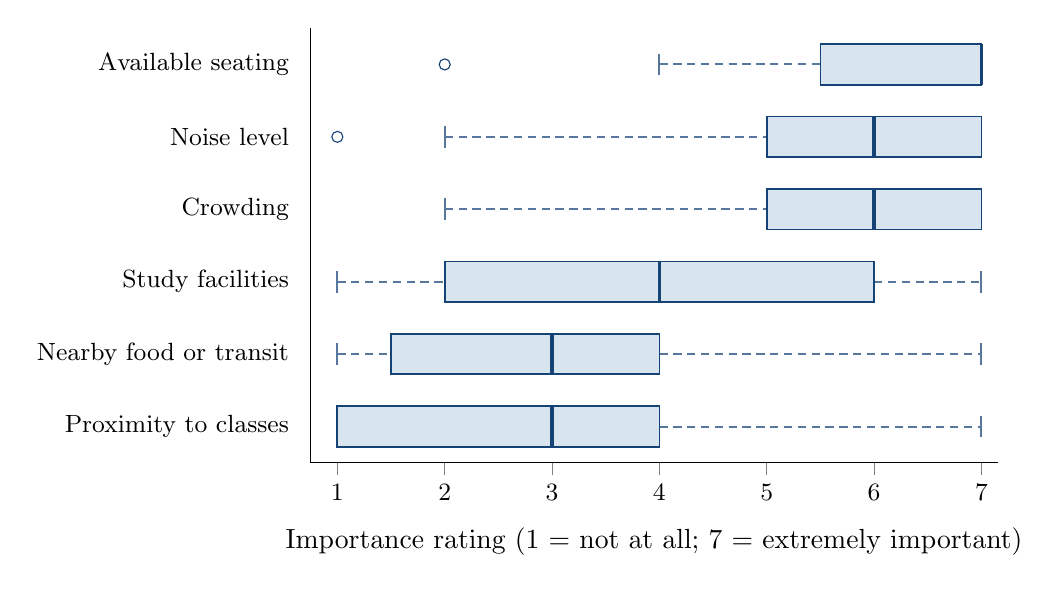
\begin{tikzpicture}
\begin{axis}[
  width=0.85\textwidth,height=7.1cm,
  xmin=0.75,xmax=7.15,ymin=0.5,ymax=6.5,
  xtick={1,2,3,4,5,6,7},ytick={1,2,3,4,5,6},
  yticklabels={Proximity to classes,Nearby food or transit,Study facilities,Crowding,Noise level,Available seating},
  xlabel={Importance rating (1 = not at all; 7 = extremely important)},
  xlabel style={yshift=-3pt},
  yticklabel style={font=\small},
  xticklabel style={font=\small},
  axis x line*=bottom,axis y line*=left,
  ytick style={draw=none},
  tick align=outside,clip=false,
  enlarge x limits=false,
  grid=none]
% The five statistics in each box use type-7 sample quartiles.
% Whiskers extend to the most extreme observations within 1.5 x IQR;
% observations beyond the whiskers are shown as open circles.
% Available seating: low=4, Q1=5.5, median=7.0, Q3=7.0, high=7
\draw[utblue!72,densely dashed,line width=0.7pt] (axis cs:4,6) -- (axis cs:5.5,6);
\draw[utblue!72,line width=0.7pt] (axis cs:4,5.85) -- (axis cs:4,6.15);
\path[draw=utblue,line width=0.65pt,fill=mutedblue!24] (axis cs:5.5,5.72) rectangle (axis cs:7,6.28);
\draw[utblue,line width=1.35pt] (axis cs:7,5.72) -- (axis cs:7,6.28);
\addplot[only marks,mark=o,mark size=2pt,draw=utblue,fill=white] coordinates {(2,6)};
% Noise level: low=2, Q1=5.0, median=6.0, Q3=7.0, high=7
\draw[utblue!72,densely dashed,line width=0.7pt] (axis cs:2,5) -- (axis cs:5,5);
\draw[utblue!72,line width=0.7pt] (axis cs:2,4.85) -- (axis cs:2,5.15);
\path[draw=utblue,line width=0.65pt,fill=mutedblue!24] (axis cs:5,4.72) rectangle (axis cs:7,5.28);
\draw[utblue,line width=1.35pt] (axis cs:6,4.72) -- (axis cs:6,5.28);
\addplot[only marks,mark=o,mark size=2pt,draw=utblue,fill=white] coordinates {(1,5)};
% Crowding: low=2, Q1=5.0, median=6.0, Q3=7.0, high=7
\draw[utblue!72,densely dashed,line width=0.7pt] (axis cs:2,4) -- (axis cs:5,4);
\draw[utblue!72,line width=0.7pt] (axis cs:2,3.85) -- (axis cs:2,4.15);
\path[draw=utblue,line width=0.65pt,fill=mutedblue!24] (axis cs:5,3.7199999999999998) rectangle (axis cs:7,4.28);
\draw[utblue,line width=1.35pt] (axis cs:6,3.7199999999999998) -- (axis cs:6,4.28);
% Study facilities: low=1, Q1=2.0, median=4.0, Q3=6.0, high=7
\draw[utblue!72,densely dashed,line width=0.7pt] (axis cs:1,3) -- (axis cs:2,3);
\draw[utblue!72,densely dashed,line width=0.7pt] (axis cs:6,3) -- (axis cs:7,3);
\draw[utblue!72,line width=0.7pt] (axis cs:1,2.85) -- (axis cs:1,3.15);
\draw[utblue!72,line width=0.7pt] (axis cs:7,2.85) -- (axis cs:7,3.15);
\path[draw=utblue,line width=0.65pt,fill=mutedblue!24] (axis cs:2,2.7199999999999998) rectangle (axis cs:6,3.2800000000000002);
\draw[utblue,line width=1.35pt] (axis cs:4,2.7199999999999998) -- (axis cs:4,3.2800000000000002);
% Nearby food or transit: low=1, Q1=1.5, median=3.0, Q3=4.0, high=7
\draw[utblue!72,densely dashed,line width=0.7pt] (axis cs:1,2) -- (axis cs:1.5,2);
\draw[utblue!72,densely dashed,line width=0.7pt] (axis cs:4,2) -- (axis cs:7,2);
\draw[utblue!72,line width=0.7pt] (axis cs:1,1.85) -- (axis cs:1,2.15);
\draw[utblue!72,line width=0.7pt] (axis cs:7,1.85) -- (axis cs:7,2.15);
\path[draw=utblue,line width=0.65pt,fill=mutedblue!24] (axis cs:1.5,1.72) rectangle (axis cs:4,2.2800000000000002);
\draw[utblue,line width=1.35pt] (axis cs:3,1.72) -- (axis cs:3,2.2800000000000002);
% Proximity to classes: low=1, Q1=1.0, median=3.0, Q3=4.0, high=7
\draw[utblue!72,densely dashed,line width=0.7pt] (axis cs:4,1) -- (axis cs:7,1);
\draw[utblue!72,line width=0.7pt] (axis cs:7,0.85) -- (axis cs:7,1.15);
\path[draw=utblue,line width=0.65pt,fill=mutedblue!24] (axis cs:1,0.72) rectangle (axis cs:4,1.28);
\draw[utblue,line width=1.35pt] (axis cs:3,0.72) -- (axis cs:3,1.28);
\end{axis}
\end{tikzpicture}
\caption{Importance ratings for the six study-environment factors ($n = 55$). The boxplots show \\ the median, interquartile range (IQR), whiskers, and potential outliers for each factor.}
\label{fig:importance}
\end{figure}
\section{Where do students usually study, and is it their first choice? (RQ2)}

As shown in Table 2, home or residence was the most common study location, with 35 out of 55 students (63.6\%) selecting it. The UTM Library was the second most common choice, with 14 students (25.5\%) studying on either the basement/main level or upper floors. The remaining students reported studying in other campus spaces or off-campus locations.

When asked how often their usual study location was also their first choice, 53 students (96.4\%) selected often, very often, or always. However, only 19 students (34.5\%) selected always. This suggests that while most students generally study where they prefer, their usual location is not necessarily their first choice every time.

Overall, the results indicate that studying at home is the most common arrangement among respondents, and most students are generally satisfied with their usual study location.

\begin{table}[H]\centering\small
\label{tab:usual}
\begin{tabular}{@{}p{9cm}rr@{}}\toprule
Location & Count & Percent\\\midrule
Home/residence & 35 & 63.6\%\\
UTM Library: basement/main level & 8 & 14.5\%\\
UTM Library: upper floors & 6 & 10.9\%\\
Davis study/silent rooms & 2 & 3.6\%\\
Another UTM campus space & 3 & 5.5\%\\
Other: Robarts Library (coded write-in) & 1 & 1.8\%\\\midrule
Total & 55 & 100.0\%\\\bottomrule
\end{tabular}
\caption{Number and percentage of students who reported each location as their usual study location ($n = 55$).}
\end{table}

\section{Does location differ by academic task? (RQ3)}
To examine whether study location differs depending on the type of academic task, we compared where students completed their most recent study session. We grouped individual studying and individual assignments into one category ($n = 50$), and collaborative studying and group assignments into another ($n = 5$). Study locations were also grouped into home/residence, UTM Library, and other locations to make the comparison easier.

\begin{table}[H]\centering\small
\label{tab:cross}
\begin{tabular}{@{}lrrrr@{}}\toprule
Task type & Home/residence & UTM Library & Other locations & Total\\\midrule
Individual & 32 (64.0\%) & 10 (20.0\%) & 8 (16.0\%) & 50\\
Collaborative & 3 (60.0\%) & 0 (0.0\%) & 2 (40.0\%) & 5\\\midrule
Total & 35 & 10 & 10 & 55\\\bottomrule\end{tabular}
\caption{Number and percentage of respondents studying at each location during their \\most recent study session, grouped by individual and collaborative work (n = 55).\\ Percentages are calculated within each task category.}
\end{table}

As shown in Table 3, 64.0\% of students completing individual work studied at home, compared to 60.0\% of those completing collaborative work. Students completing collaborative work were also more likely to study in other locations (40.0\%) compared to those completing individual work (16.0\%). However, only five respondents reported collaborative work, so these differences should be interpreted cautiously.

We initially considered a Chi-square test of independence to examine the relationship between task type and study location. However, Table 4 shows that three of the six expected frequencies were below 5, meaning the Chi-square test assumptions were not met. We therefore used Fisher's exact test, which is more appropriate for our small sample sizes.

\begin{table}[H]\centering\small
\label{tab:expected}
\begin{tabular}{@{}lrrr@{}}\toprule
Task type & Home/residence & UTM Library & Other locations\\\midrule
Individual & 31.82 & 9.09 & 9.09\\
Collaborative & 3.18 & 0.91 & 0.91\\\bottomrule\end{tabular}
\caption{Expected frequencies for each combination of academic task type and study location under the assumption that the two variables are independent.}
\end{table}

The test produced a \textit{p} = 0.418. Since this is greater than the significance level of 0.05, we do not have sufficient evidence to conclude that study location differs depending on the type of academic task. However, with only five students reporting collaborative work, our results may not capture differences that exist between the two groups.


\section{What barriers prevent regular preferred-location use? (RQ4)}
To identify the barriers students face when using their preferred study location, we focused on respondents who reported being able to use that location only sometimes or less often (ratings of 1–4). This left us with five respondents. Since students could select multiple barriers, the percentages do not necessarily add up to 100\%.

\begin{table}[H]\centering\footnotesize
\label{tab:primarybarriers}
\begin{tabular}{@{}p{5.7cm}rrr@{}}\toprule
Barrier & Count (\%) & Bootstrap CI & Wilson CI\\\midrule
Not enough available seating & 3 (60.0\%) & 20.0--100.0 & 23.1--88.2\\
Space too crowded & 2 (40.0\%) & 0.0--80.0 & 11.8--76.9\\
Noise level too high & 2 (40.0\%) & 0.0--80.0 & 11.8--76.9\\
Travel time or distance & 2 (40.0\%) & 0.0--80.0 & 11.8--76.9\\
Limited opening hours & 3 (60.0\%) & 20.0--100.0 & 23.1--88.2\\
Transportation difficulties & 1 (20.0\%) & 0.0--60.0 & 3.6--62.4\\
Unavailable study facilities & 0 (0.0\%) & 0.0--0.0 & 0.0--43.4\\
Need to remain near classes & 1 (20.0\%) & 0.0--60.0 & 3.6--62.4\\
Temperature/air quality (write-in) & 1 (20.0\%) & 0.0--60.0 & 3.6--62.4\\\bottomrule\end{tabular}
\caption{Barriers among respondents with preferred-location access ratings 1--4 ($n=5$). Proportions are observed shares; percentile bootstrap and Wilson intervals are 95\% ranges (in percentages).}
\end{table}

As shown in Table 5, lack of available seating and limited opening hours were the most commonly reported barriers, with three out of five students (60\%) selecting each. Crowding, noise, and travel time were also reported by two students each (40\%).

We used bootstrapping with 20,000 resamples to calculate 95\% confidence intervals for each barrier proportion. These intervals were generally wide because our analysis included only five students. This means that while seating and opening hours were the most frequently reported barriers in this group, we cannot confidently conclude that they are the most common barriers among all STA304 students.

\begin{table}[H]\centering\small
\label{tab:sensitivity}
\begin{tabular}{@{}p{7cm}rrr@{}}\toprule
Barrier & Scores 1--4 ($n=5$) & 1--5 ($n=16$) & 1--6 ($n=28$)\\\midrule
Not enough available seating & 3 (60.0\%) & 8 (50.0\%) & 14 (50.0\%)\\
Space too crowded & 2 (40.0\%) & 6 (37.5\%) & 10 (35.7\%)\\
Noise level too high & 2 (40.0\%) & 6 (37.5\%) & 8 (28.6\%)\\
Travel time or distance & 2 (40.0\%) & 7 (43.8\%) & 10 (35.7\%)\\
Limited opening hours & 3 (60.0\%) & 6 (37.5\%) & 7 (25.0\%)\\
Transportation difficulties & 1 (20.0\%) & 4 (25.0\%) & 6 (21.4\%)\\
Unavailable study facilities & 0 (0.0\%) & 1 (6.2\%) & 4 (14.3\%)\\
Need to remain near classes & 1 (20.0\%) & 4 (25.0\%) & 7 (25.0\%)\\
Temperature/air quality & 1 (20.0\%) & 1 (6.2\%) & 1 (3.6\%)\\\bottomrule\end{tabular}
\caption{Comparison of reported barrier percentages using three definitions of limited access to a preferred study location (ratings of 1–4, 1–5, and 1–6).}
\end{table}

We also considered how the results would change if we included students who could access their preferred location more frequently. As shown in Table 6, seating remained one of the most common barriers across all three groups. However, the percentage reporting limited opening hours decreased from 60\% to 25\% when students with access ratings of 5 and 6 were included. This shows that our findings depend partly on how we define irregular access to a preferred study location.


\section{Model Assumptions}

Our analysis focuses on proportions, categorical variables, and bootstrapping rather than linear regression. Therefore, the assumptions of normally distributed residuals and equal error variances do not apply to the statistical methods we used.

For RQ3, we checked the expected frequencies before performing the Chi-square test of independence. As discussed in Section 5, several expected counts were below 5, so we used Fisher's exact test instead. This allowed us to examine the relationship between academic task type and study location without relying on the Chi-square approximation.

For RQ4, we used bootstrapping to estimate confidence intervals for the reported barriers. Since only five respondents met our definition of irregular access, the bootstrap estimates were limited by the small sample size. We also calculated Wilson confidence intervals to provide another measure of uncertainty, particularly for barriers that were not reported by any respondents.

Although our methods do not require normally distributed residuals or equal error variances, they still have limitations. In particular, the small sample size for RQ4 and the voluntary nature of our survey affect how confidently we can generalize our findings to all STA304 students.


\section{Overall interpretation and limitations}
Our results suggest that students place the most importance on having enough seating, a suitable noise level, and a less crowded environment when choosing where to study. Home or residence was the most common study location among respondents, and most students reported that their usual study location was also their first choice at least often.

We did not find sufficient evidence of a relationship between academic task type and study location. However, only five respondents reported collaborative work, which limits our ability to identify differences between individual and group studying. For students who could not regularly access their preferred study location, lack of seating and limited opening hours were the most commonly reported barriers.

There are several limitations to consider. Since participation in our survey was voluntary, our sample may not fully represent all students enrolled in STA304H5F. The small number of respondents in certain groups, particularly for RQ3 and RQ4, also makes it difficult to draw strong conclusions. Additionally, our findings are based on students' self-reported responses rather than direct observations of their study habits.

Overall, our findings provide some insight into the study preferences and challenges reported by STA304 students, but they should not be generalized to the entire course population without further research.

\appendix
\section{Categorical frequency tables}\label{app:freq}
\begin{table}[H]\centering\small
\begin{tabular}{@{}p{3cm}p{7.7cm}r@{}}\toprule
Variable & Category & $n$ (\%)\\\midrule
Recent location & Home/residence & 35 (63.6\%)\\
 & UTM Library: basement/lower & 6 (10.9\%)\\
 & UTM Library: first floor & 2 (3.6\%)\\
 & UTM Library: upper floors & 2 (3.6\%)\\
 & Davis study/silent rooms & 1 (1.8\%)\\
 & Other UTM campus space & 8 (14.5\%)\\
 & Another off-campus location & 1 (1.8\%)\\\midrule
Recent task & Individual studying/reading & 28 (50.9\%)\\
 & Individual assignment/project & 22 (40.0\%)\\
 & Collaborative studying & 3 (5.5\%)\\
 & Collaborative assignment/project & 2 (3.6\%)\\\bottomrule\end{tabular}
 \caption{Recent study locations and work types, at the original level of detail ($n=55$).}
 \end{table}

\begin{table}[H]\centering\small
\begin{tabular}{@{}p{7.3cm}rr@{}}\toprule
Barrier & Selected & Not selected\\\midrule
No barriers & 15 (27.3\%) & 40 (72.7\%)\\
Not enough seating & 17 (30.9\%) & 38 (69.1\%)\\
Too crowded & 16 (29.1\%) & 39 (70.9\%)\\
Noise too high & 13 (23.6\%) & 42 (76.4\%)\\
Travel time or distance & 12 (21.8\%) & 43 (78.2\%)\\
Limited opening hours & 8 (14.5\%) & 47 (85.5\%)\\
Transportation difficulties & 8 (14.5\%) & 47 (85.5\%)\\
Required facilities unavailable & 7 (12.7\%) & 48 (87.3\%)\\
Need to remain near classes & 11 (20.0\%) & 44 (80.0\%)\\
Temperature or air quality & 1 (1.8\%) & 54 (98.2\%)\\\bottomrule\end{tabular}
\caption{All binary barrier variables, plus the mutually exclusive ``no barriers'' choice, for the full 55 responses. Selection percentages need not sum to 100\%.}
\end{table}

The single usual-location write-in was coded 1 (Robarts Library), versus 54 coded 0 (no write-in); the single barrier write-in was coded 1 (temperature/air quality), versus 54 coded 0. The raw texts and corresponding numeric codes represent the same two observations and are not counted twice. Course IDs are identifiers rather than outcomes.

\section{Complete frequency distributions for the ordinal ratings}\label{app:ratings}
\begin{table}[H]\centering\scriptsize
\begin{tabular}{@{}p{6.6cm}rrrrrrr@{}}\toprule
Rating & 1 & 2 & 3 & 4 & 5 & 6 & 7\\\midrule
Usual location as first choice & 0 & 0 & 0 & 2 & 10 & 24 & 19\\
Importance: noise level & 2 & 1 & 2 & 7 & 11 & 12 & 20\\
Importance: available seating & 0 & 1 & 0 & 4 & 9 & 13 & 28\\
Importance: crowding & 0 & 5 & 3 & 5 & 14 & 9 & 19\\
Importance: proximity to classes & 15 & 10 & 10 & 9 & 3 & 2 & 6\\
Importance: food/transit proximity & 14 & 11 & 6 & 11 & 5 & 3 & 5\\
Importance: study facilities & 6 & 11 & 4 & 7 & 5 & 10 & 12\\
Access to preferred location & 0 & 0 & 1 & 4 & 11 & 12 & 27\\
Changing planned location & 4 & 14 & 7 & 15 & 10 & 4 & 1\\\bottomrule\end{tabular}
\caption{Counts at every rating level (1--7), including unobserved levels. Each row sums to 55.}
\end{table}

Importance scale: 1 = not at all important through 7 = extremely important. Frequency scale: 1 = never through 7 = always. For these items there are no missing numerical responses; empty write-in fields indicate no write-in, not missing Likert responses.


\clearpage
\section{Complete R analysis code}\label{app:code}

\begin{lstlisting}[style=rsource]

# STA304H5F, Part 4: Reproducible Exploratory Analysis

# Install easystats once if needed:
# install.packages("easystats")

library(easystats)

# Load data
d <- read.csv("STA304_dataset.csv",
              check.names = FALSE,
              nrows = 55)

stopifnot(nrow(d) == 55)

# Descriptive statistics for all quantitative variables
ratings <- c("usual_is_first_choice", "imp_noise", "imp_seating",
             "imp_crowding", "imp_class_proximity", "imp_food_transit",
             "imp_facilities", "preferred_location_access",
             "change_location_frequency")

stopifnot(!anyNA(d[ratings]))

print(datawizard::describe_distribution(
  d[ratings], centrality = "all"
))

print(datawizard::data_tabulate(d, "recent_work_type"))

summary_scores <- do.call(rbind, lapply(ratings, function(v) {
  x <- d[[v]]
  data.frame(item = v, n = length(x),
             mean = mean(x), median = median(x),
             sd = sd(x), IQR = IQR(x, type = 7),
             min = min(x), max = max(x))
}))

print(summary_scores)

# Frequencies for all 1-7 response scales
for (v in ratings) {
  print(table(factor(d[[v]], levels = 1:7)))
}

# Frequencies for categorical variables
for (v in c("usual_location", "recent_location",
            "recent_work_type")) {
  print(table(d[[v]]))
}

# Binary indicators for barriers and thematic codes
barriers <- c("barrier_seating", "barrier_crowded",
              "barrier_noise", "barrier_travel",
              "barrier_hours", "barrier_transport",
              "barrier_facilities", "barrier_classes",
              "barrier_other_code")

for (v in c("usual_location_other_code",
            "no_barriers", barriers)) {
  print(table(factor(d[[v]], levels = 0:1)))
}

# --------------------------------------------------
# RQ1: Importance of study-environment factors
# --------------------------------------------------

items <- list(
  "Proximity to classes" = d$imp_class_proximity,
  "Nearby food or transit" = d$imp_food_transit,
  "Study facilities" = d$imp_facilities,
  "Crowding" = d$imp_crowding,
  "Noise level" = d$imp_noise,
  "Available seating" = d$imp_seating
)

boxplot(items,
        horizontal = TRUE,
        outline = TRUE,
        xlim = c(1, 7),
        xlab = "Importance rating (1 = not at all; 7 = extremely important)")

# --------------------------------------------------
# RQ2: Usual study locations and first choice
# --------------------------------------------------

print(prop.table(table(d$usual_location)))

# Exact binomial confidence intervals
print(binom.test(sum(d$usual_location == 1),
                 nrow(d))$conf.int)

print(binom.test(sum(d$usual_is_first_choice >= 5),
                 nrow(d))$conf.int)

print(binom.test(sum(d$usual_is_first_choice == 7),
                 nrow(d))$conf.int)

# --------------------------------------------------
# RQ3: Study location versus academic task type
# --------------------------------------------------

task <- factor(
  ifelse(d$recent_work_type <= 2,
         "Individual", "Collaborative"),
  levels = c("Individual", "Collaborative")
)

loc <- factor(
  ifelse(d$recent_location == 1,
         "Home/residence",
         ifelse(d$recent_location %in% 2:4,
                "UTM Library", "Other")),
  levels = c("Home/residence", "UTM Library", "Other")
)

# Contingency table
ct <- table(task, loc)
print(ct)

# Row proportions
print(prop.table(ct, 1))

# Check Chi-square assumptions
chi <- suppressWarnings(
  chisq.test(ct, correct = FALSE)
)

print(chi)
print(chi$expected)

# Fisher's exact test for sparse expected counts
print(fisher.test(ct))

# Sensitivity analysis with original location categories
ct_original <- table(
  task,
  factor(d$recent_location, levels = 1:7)
)

print(fisher.test(ct_original, workspace = 2e7))

# --------------------------------------------------
# RQ4: Barriers to preferred study locations
# --------------------------------------------------

# Primary group: access scores 1-4
primary <- d[d$preferred_location_access <= 4, ,
             drop = FALSE]

B <- as.matrix(primary[barriers])

stopifnot(nrow(B) == 5)

# Bootstrap 95% confidence intervals
set.seed(20261021)
nboot <- 20000

boot <- replicate(nboot, {
  i <- sample.int(nrow(B), nrow(B), replace = TRUE)
  colMeans(B[i, , drop = FALSE])
})

bootstrap_results <- data.frame(
  barrier = barriers,
  selected = colSums(B),
  percentage = 100 * colMeans(B),
  low = 100 * apply(boot, 1, quantile,
                    probs = 0.025),
  high = 100 * apply(boot, 1, quantile,
                     probs = 0.975)
)

print(bootstrap_results)

# Wilson 95% confidence intervals
wilson <- function(k, n, z = qnorm(0.975)) {
  p <- k / n
  a <- 1 + z^2 / n

  lower <- (p + z^2/(2*n) -
            z*sqrt(p*(1-p)/n + z^2/(4*n^2))) / a

  upper <- (p + z^2/(2*n) +
            z*sqrt(p*(1-p)/n + z^2/(4*n^2))) / a

  c(lower, upper)
}

wilson_results <- t(vapply(
  colSums(B),
  wilson,
  numeric(2),
  n = nrow(B)
))

print(wilson_results)

# Sensitivity analysis for access thresholds
for (cutoff in c(4, 5, 6)) {

  eligible <- d[
    d$preferred_location_access <= cutoff, ,
    drop = FALSE
  ]

  print(data.frame(
    cutoff = cutoff,
    n = nrow(eligible),
    barrier = barriers,
    yes = colSums(eligible[barriers]),
    pct = 100 * colMeans(eligible[barriers])
  ))
}

\end{lstlisting}

\end{document}